\documentclass[12pt]{article}
\usepackage{standalone}
\usepackage{graphicx}

% Nom du sommaire
\renewcommand*\contentsname{Sommaire}

\begin{document}

% Page de Titre
\begin{titlepage}
    \begin{center}
        \textbf{Rapport de Génie Logiciel} \\
        \vspace{0.5cm}
        Titouan Loiseau et Baptiste Marchand \\
        4A SAGI - TD2 \\
        \vspace{5cm}

        
\includegraphics[height=3cm]{img/Polytech_Angers.png} \\
        
\includegraphics[height=2cm]{img/git.png}
        
\includegraphics[height=2cm]{img/junit.png}
        
\includegraphics[height=2cm]{img/uml.png}
    \end{center}
\end{titlepage}

% Sommaire
\tableofcontents
\pagebreak

% Introduction
\addcontentsline{toc}{section}{Introduction}
\section*{Introduction}

% Exercice 1
\section{Exercice 1}
\subsection{Q1}

La figure~\ref{UC1} présente le premier diagramme de classes imaginé. 

\begin{figure}[h]
    \centering
    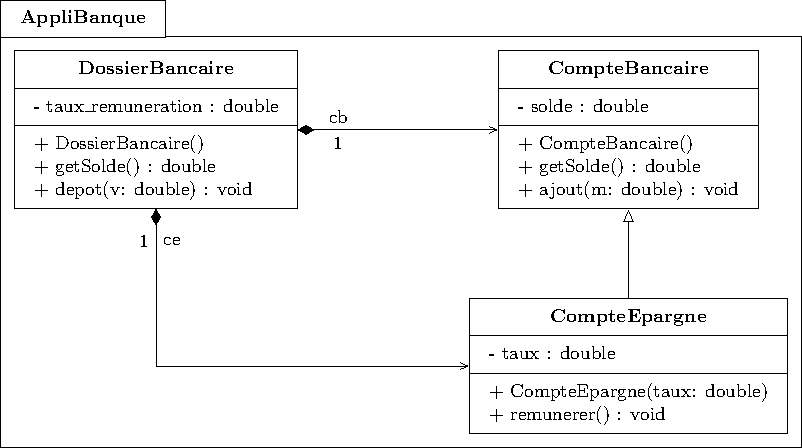
\includegraphics{Diagrammes/UML_UC1.pdf}
    \caption{Diagramme de classes\label{UC1}}
\end{figure}


\subsection{Q2}

La figure~\ref{US1} présente le premier diagramme de classes imaginé. 
\begin{figure}[h]
    \centering
    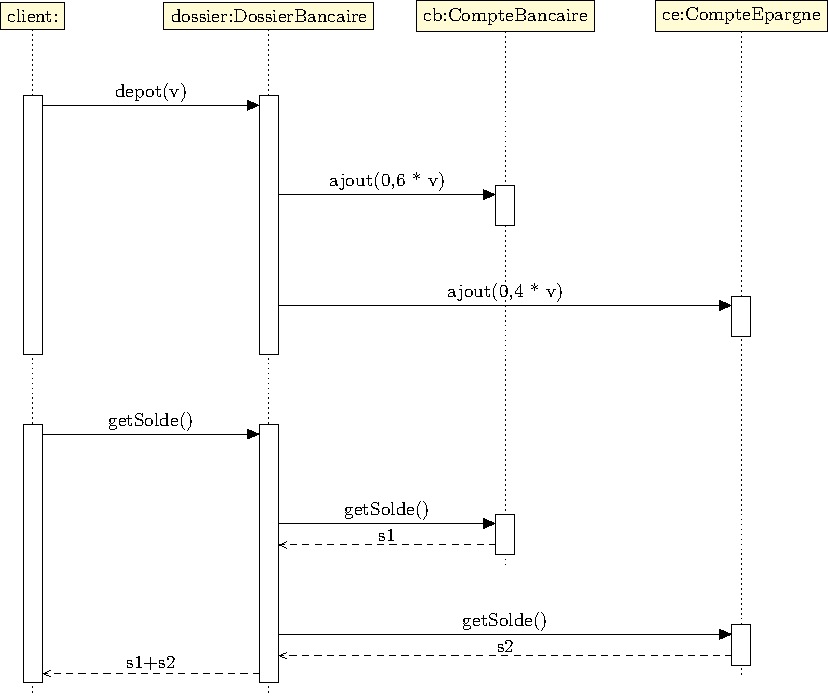
\includegraphics{Diagrammes/UML_US1.pdf}
    \caption{Diagramme de séquence\label{US1}}
\end{figure}


\subsection{Q3}

En plus des diagrammes précédents, on peut faire un diragramme d'objets modélisant l'état du programme après l'instanciation de l'objet de la classe DossierBancaire.
La figure~\ref{UO1} présente un tel diagramme. 
\begin{figure}[h]
    \centering
    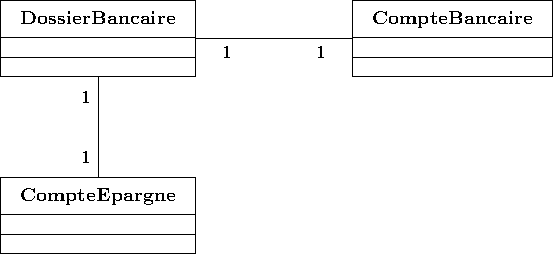
\includegraphics{Diagrammes/UML_UO1.pdf}
    \caption{Diagramme d\textquotesingle objets\label{UO1}}
\end{figure}
\end{document}